\documentclass[output=paper]{LSP/langsci} 
\ChapterDOI{10.5281/zenodo.1441347}

\author{João Antônio de Moraes\affiliation{Universidade Federal do Rio de Janeiro, CNPq}\lastand 
Albert Rilliard\affiliation{LIMSI, CNRS, Université Paris-Saclay}
}

\title{Describing the intonation of speech acts in Brazilian Portuguese: Methodological aspects}
\shorttitlerunninghead{Describing the intonation of speech acts in Brazilian Portuguese } 
 

\abstract{This chapter details a methodology based on the notion of close-copy and equivalent-copy \citep{hart1991jasa}, showing how systematic modifications of pitch contours using resynthesis techniques allow for testing the phonological and/or expressive nature of prosodic changes for speech-act performances. The methodology is illustrated with examples of prosodically performed speech acts in Brazilian Portuguese. A perception test shows that listeners are able to discriminate between these speech acts on prosodic cues alone. Then systematic modifications of their pitch contours are detailed and synthesized. Perceptual validation of these productions shows: (1) the relative importance of pitch versus intensity and duration for these expressions; and (2) the importance of each turning point along the stylized pitch contour, both in terms of pitch height and segmental anchoring. The results support the need for three pitch levels for the phonological description of speech acts in Brazilian Portuguese. They also show the importance of the segmental anchoring of valleys for the acceptability of contours.
}

% {Keywords:} intonation, speech acts, prosodic stylization,  perception, resynthesis.

\maketitle

\begin{document}
\label{chap:mor}\label{ch:7}

\section{Introduction} 
\label{introduction}



One of the central functions of intonation/prosody, along with phrasing and focalization, is the expression of the illocutionary force of utterances, which characterizes them as different speech acts. 
Classical works on the Speech Act theory \citep{Austin1962,Searle1969,Vanderveken1990,Alston2000} have based their inventories of speech acts mostly on the existence of performative verbs. 
These works have relied upon written forms of language, and account for introspective representations of hypothetical examples. 
Within such approaches, prosody has been only incidentally mentioned as a potential tool in speech act performances. 
More recent works have asserted the importance of including oral and unscripted language productions for the description of speech acts \citep{Cresti2000,Moneglia2011,Raso2012,TamotoAndKawabata}.  
Such an approach for describing language in its actual use puts emphasis on the role of intonation in conveying speech acts. 
In doing so, it notably shows the relevance of prosodic variants in the performance of sets of illocutions. 
This is done in situations where no other factors (whether morphosyntactic or lexical) can explain the given illocutionary force that is carried by an utterance, other than the peculiarities of its prosody.
In Brazilian Portuguese, for instance, a number of directive acts may be distinguished by means of their prosodic patterns; a directive act is here understood as an attempt by the speaker to induce an action from the hearer (\citealt{Searle1979}).%; see \citealt{Sakakibara1979} for a critical account on Searle 1976 = 1979).


Works such as those pursued in the framework of the C-ORAL-ROM corpus (\citealt{Cresti2000,Moneglia2011,Raso2012}) or by other research groups (e.g., \citealt{fontaney1991question,culpeper2003impoliteness,Moraes12}) provide significant sources of knowledge on speech act performances, especially due to the ``spontaneous'' nature of the data on which they base their analysis (on this notion of ``spontaneous speech'', cf. \citealt{blanche1999franccais}). 
Because they study in detail occurrences of speech observed in context, they may derive and model their occurrence context, the relations between the speaker and the interlocutors, the speech act aims, etc. (see \citealt{kohler2004pragmatic}).
This allows, to some extent, for developing models of interactions based on the observation of performances unconstrained by theoretical or a priori views (but see \citealt{Wagner.2015}, for another view on data selection).  
On the other hand, recognized features of such in-the-field speech productions are also characterized by low quality of the acoustic signal (compared to ``lab speech''), as well as by unconstrained utterances. 
The use of such material makes it more difficult to perform strict comparisons of acoustic changes across studied categories. 
On the contrary, and as defended notably by \citet{Xu2010}, lab speech presents characteristics that are not found in unconstrained productions (such as strict control over the sources of variation, crucial for pursuing controlled psycholinguistic experimentation). 
Such properties of lab speech are primarily useful for (in)validating theoretical proposals, but it is desirable that various studies could be produced on the basis of typologically different types of spoken productions \citep{Wagner.2015}.

We thus defend here the view that out-of-the-lab speech is of an indisputable interest in developing theories through the observation of recurrent patterns in the actual use of speech during situations of communication, and that such theoretical proposals may usefully be tested in controlled experimental settings (as has been done for example by \citealt{GussenhovenChen2000,Boula2002,house2005phrase,dimperio2010alignment,Vanrell2013certainty,Borras-Comes2015}). 
Unconstrained recordings (in the Labovian tradition) may lead to observations that were not observed or described on the basis of constrained recordings (see for example the main perceptual correlates of smiled speech in \citealt{Emond2013}, which contrast with those described by \citealt{Tartter1980}). 
Lab speech, by its very nature of controlled recordings, reduces the variability of speech; the conclusions of studies based on such material thus have to be correlated to observations of unconstrained performances. 
This is notably true for inter-speaker variability (or said another way, of idiosyncratic strategies) that may be downplayed (or enhanced) by laboratory approaches based on a few subjects. 
Meanwhile, a careful selection of controlled parameters allows for repeatable experiments; the key here is in a number of studies that can vary some characteristics (or style, to follow the terminology in \citealt{Wagner.2015}) of the recordings (type and structure of sentences, list and nature of speech acts, speakers' gender or dialectal origin, etc.), so as to gradually improve the understanding of the extent to which such cues may convey a given communicative function. 
Recurrent observations of a phenomenon back and forth in both controlled and uncontrolled circumstances are the best way to assert the robustness of theoretical observations -- \citet{house2005phrase} being an example of such a methodology linking spontaneous and controlled utterances (see also \citeauthor{Peskova.2018}, this volume, for similar observations).

The intonation of Portuguese has been well studied in the last decade, for both European Portuguese (EP) and Brazillian Portuguese (BP) varieties, including in its illocutionary dimensions, with works on the expressions of orders, requests, vocatives, or different kinds of questions, etc. \citep{moraes2008pitch,Frota2014,frotaPrieto2015,FrotaAndMoraes2016}, or even from an explicit regional perspective \citep{frota2015portuguese}. 
On the prosody of directive acts, and especially on the distinction between orders and requests, a number of studies have been done for BP \citep{Bodolay2009,Queiroz2011,Rocha2013,Rocha2016}, and fewer for the EP variety \citep{fale2007imperatives}.
Previous works have shown that the prosodic patterns of such speech acts not only have different prosodic characteristics \citep{fale2007imperatives}, but are also recognized by hearers in a consistent way \citep{veliz2004intonational,moraes2008pitch,moraes2014}.\largerpage[-1]

This paper describes a methodological process that allows the evaluation of the relative contribution of acoustic correlates of prosody, and the prototypicality of intonation contours, for the performance of a set of speech acts. 
To this aim, a resynthesis technique (implemented in Praat, \citealt{Boersma.praat}), based on stylized contours, is used to systematically change some aspects of the prosodic characteristics of utterances. 
The perception of these controlled systematic changes allows for the discussion of modifications that challenge the interpretations of speech acts versus those that merely affect the quality of the perceived pitch contour (in the line of works such as  \citealt{Uldall1960,fonagy1972}; and \citealt{house2005phrase}). 
Being decoded and interpreted by listeners, such prosodic modifications change the meaning of the verbal content, participating in the communicative meaning \citep{Mahadin2011,nadeu2011pitch,portes2014dialogical,gonzalez2015gestural}. 
Hence, by modifying the melodic contours for the pitch target's height and temporal alignment, and observing the perceptual effects of each change, we intend to show how this approach allows an evaluation of the extent to which changes are acceptable, that is, those that still carry a similar meaning as the original vs. changes that either bar access to the original speech act or change its interpretation. 
Changes of interpretation and acceptability address differences in the phonological meaning of prosodic contours, whereas changes of their perceived quality are merely circumstantial and/or expressive.
In order to support the description of the process and give examples of possible findings, the paper bases the description of the method on a set of directive speech acts produced by speakers of Brazilian Portuguese from the Rio de Janeiro variety.
As the paper focuses on the methodology and not on the linguistic description, only a restricted discussion will be given of these speech acts in this language variety (referring the interested reader to papers detailing these aspects), compared to other varieties of Portuguese, or other languages (Romance or not).
Similarly, the authors believe that such an experimental process allows the researcher to tackle prosodic variation at a very early level, and then to interpret the phonological significance of some of the observed variants.
For this reason, and before reaching strong conclusions, the experimental method will be applied to a variety of utterances from speakers of various regional and sociocultural origins.
For the same reason, it is thought to be inconvenient to describe the observed speech acts using phonological tools before evaluating the distinctive nature of the variants.


This paper first describes a set of speech acts and their prosodic variation (Section \ref{corpus:phonetic}), before presenting the concept of close-copy stylization (Section \ref{corpus:CC}) aimed at keeping only perceptually relevant intonational variation for the targeted function; other prosodic parameters are described in Section \ref{corpus:importance}. The perceptual evaluation of  systematic changes introduced in such a close-copy stylization is then presented to show how experimental processes allow for the identification of relevant patterns for the various illocutionary performances under study (Section \ref{perception}). The presented data are discussed in Section \ref{discussion}, before concluding on the pros and cons of this approach (Section \ref{conclusions}).


\section{A corpus of seven speech acts}
\label{corpus}
\subsection{Phonetic description}
\label{corpus:phonetic}

A corpus of 462 utterances, corresponding to seven speech acts, was recorded by two Brazilian Portuguese speakers (one female and one male) from Rio de Janeiro. 
We chose to record two speakers so as to capture some of the inter-speaker variation linked to the varying strategies allowed in the production of such speech acts. 
The perceptual validation of the speakers' productions shows that all were recognized (cf. infra), if differences in their performances were also observed.
The targeted speech acts are labelled in BP as follows: \textit{asserção} (`statement'), \textit{interrogação} (`yes/no question'), \textit{ordem} (`order'), \textit{desafio} (`threat', `challenge'), \textit{alerta} (`warning'), \textit{sugestão} (`suggestion', `advice'), and \textit{pedido} (`request'); the Brazilian Portuguese terms will be kept in the chapter to avoid misinterpretations based on the imperfect English translations. 
To clarify these terms, it is worth saying, following \citet{Searle1979}, that in the speech acts \textit{ordem} and \textit{pedido}, speaker S wants the hearer H to perform action A. 
In the case of \textit{ordem}, S has a social position of authority over H and uses it while performing this speech act. 
In contrast, in \textit{pedido}, S does not use or does not have a higher social position, while performing this speech act. 
In the \textit{sugestão}, S believes A will benefit H, ``advising'' being telling someone what is best for her or him. 
In the \textit{alerta}, S believes something that may not be in H's best interest could happen in case H would not do A, so S urges H to perform A for H's own good.
In the \textit{desafio}, S doesn't want H to perform A, and dares H to do so; in this sense, it is a sort of ironic order, as S wants the reverse of what she/he says, and threatens H in case she/he performs A. 
Finally, in the \textit{interrogação}, S asks for information, and in the \textit{asserção}, S transmits this information.


\begin{figure}

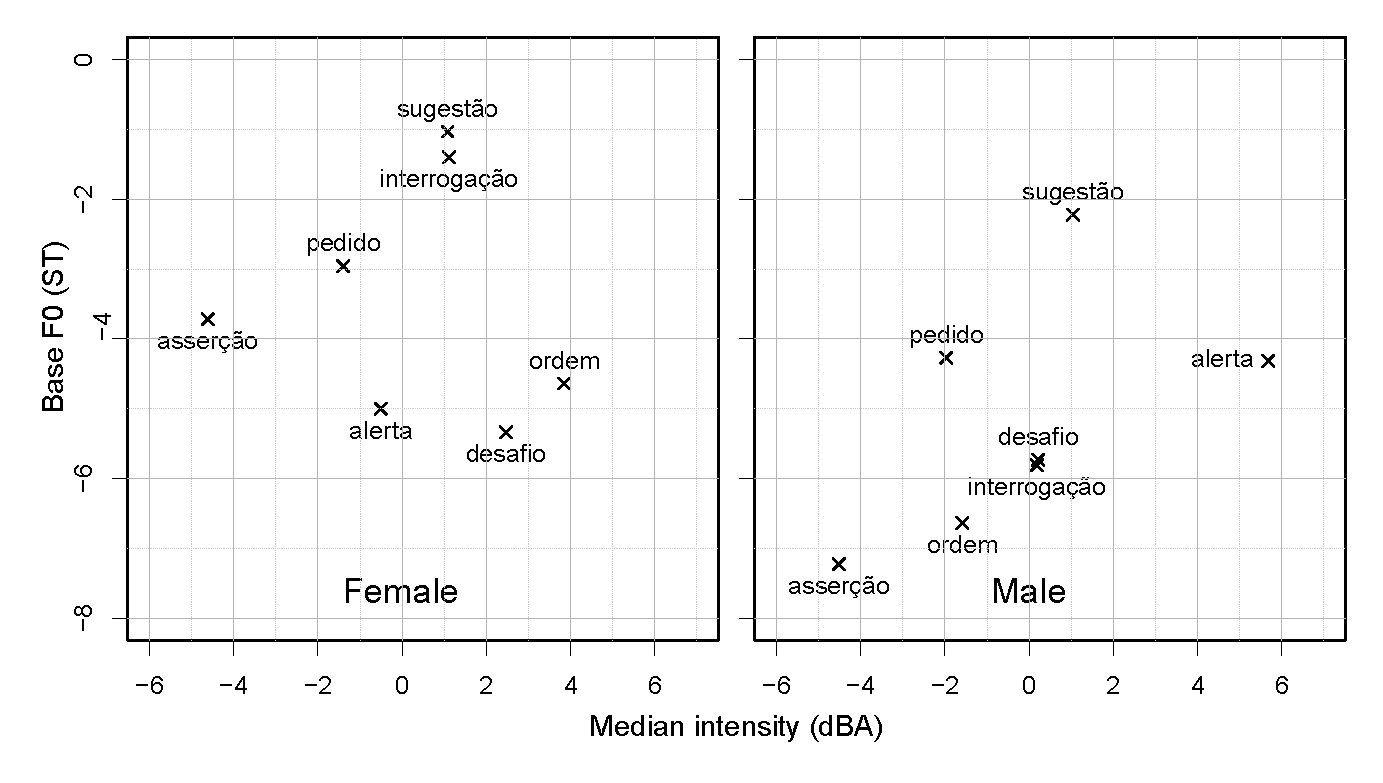
\includegraphics[width=0.99\textwidth]{figures/MOR1.eps}
\caption{Position of each speech act in the (median intensity * base F0) plane, for each speaker (left: female, right: male). }
\label{figure:f0intbase}
\end{figure}

\begin{figure}

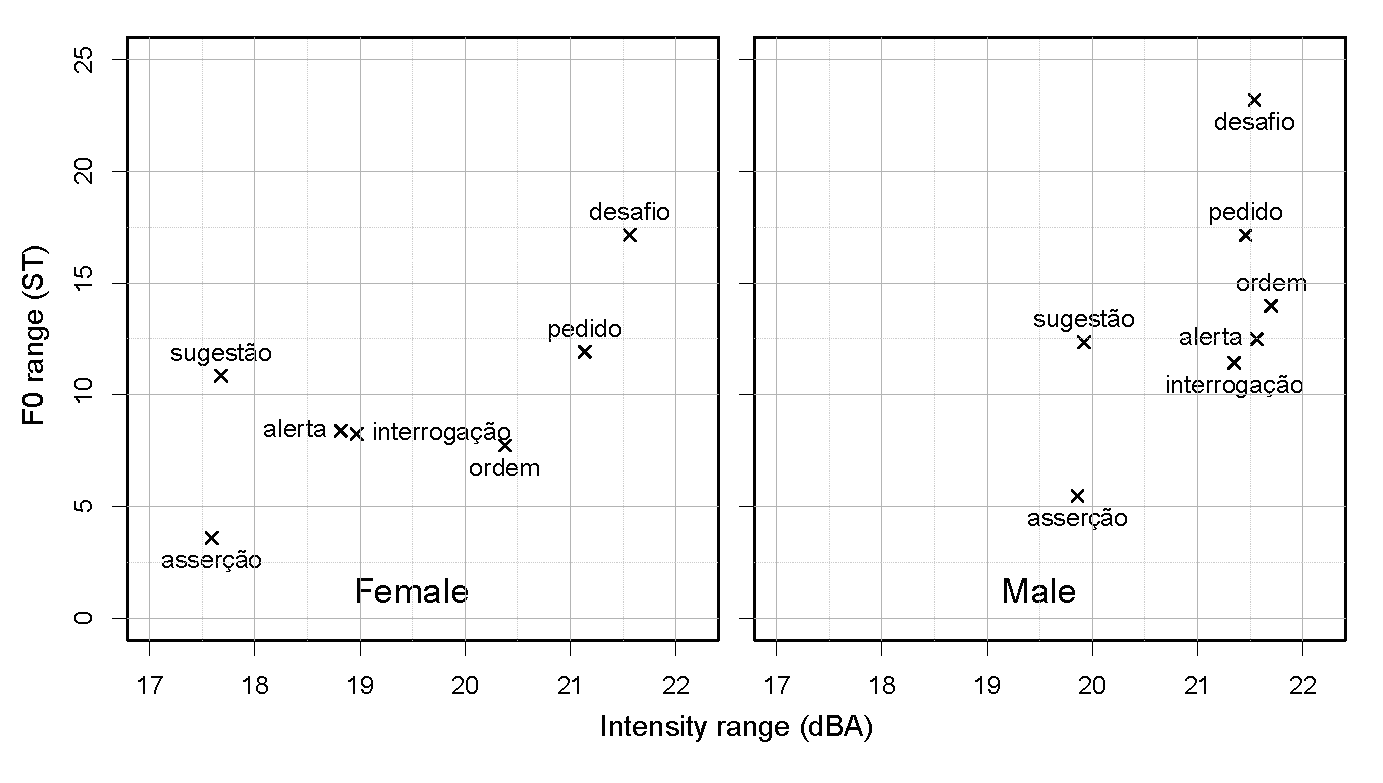
\includegraphics[width=0.99\textwidth]{figures/MOR2.eps}
\caption{Position of each speech act in the (intensity range * F0 range) plane, for each speaker (left: female, right: male).}
\label{figure:f0intrange}
\end{figure}


The mentioned speech acts were recorded on sentences of varying length: sentences of one, two, three, six, nine, and 12 syllables were used. 
For each length (except the one-syllable sentence), two sentences were proposed, ending respectively with a paroxytonic or an oxytonic word. 
This results in a set of 11 different sentences (these data are based on structures similar to one that is presented in \citealt{moraes2008pitch}, but presenting larger variation). 
Three repetitions of each of these sentences, for each speech act, were recorded by the two speakers.
Before the recordings, each speaker was presented with the seven contexts and their communicative implications. 
They were then recorded, with the speaker and an experimenter monitoring the quality of the production, and recording again in case they were not satisfied with the performance.

The fundamental frequency (F0, expressed in semitones) and A-weighted intensity (expressed in dBA) of all the sentences were extracted for each 10 milliseconds of the recorded stimuli, using Praat \citep{Boersma.praat}; values in unvoiced parts were discarded. A-weighted intensity was selected as a good correlate of the perceived vocal effort (cf. \citealt{lienard2013strength}; and similar measures in \citealt{Traunmuller2000}). 

\citet{Traunmuller1995} introduced the notion of F0 base value, linked to the perceived register of a speaker's voice and differentiated from the size of the F0 excursion in the voice. 
They estimated the base value of a speaker as 1.43 standard deviation below the speaker's mean F0. 
\citet{arantes2014}, building on this notion, have shown that the base value is a measure of preferred F0 (the frequency the speaker is more likely to use spontaneously) that stabilizes more rapidly over time compared to, for example, measures of central tendency like the mean or the median.

The F0 base value was thus estimated for each speaker and each speech act to estimate its register. 
The base value was measured as the 10th percentile of a speaker's F0 distribution in a given speech act -- a close approximation of \citet{Traunmuller1995} calculation, which also takes into account F0's skewness \citep[cf.][for a slightly different choice]{arantes2014}. 
The amplitude of pitch excursions in each speech act was estimated by calculating the difference between the 90th and the 10th percentile of F0. 
The median intensity was calculated to indicate the preferred effort used to perform a given speech act; the span of intensity (the difference between the 90th and the 10th percentiles of intensity) measures variation in intensity.
The F0 and intensity measures were corrected for speaker-specific value by subtracting the speaker-specific values of (respectively) base F0 and median intensity from the raw measures.

Figure~\ref{figure:f0intbase} presents the position of speech acts according to their median intensity and F0 base value. 
It thus represents the preferred pitch and average effort required for each speech act. 
Figure~\ref{figure:f0intrange} presents the speech act's span in pitch and intensity -- thus representing the acoustic variation linked to these expressions.\largerpage[-1]

Figure~\ref{figure:f0intrange} shows that both speakers are highly coherent in the prosodic changes they produce for each speech act: The distribution of F0 and intensity spans are the same -- even if the male speaker uses a reduced span of intensity compared to the female speaker. 
In that figure, \textit{asserção} (`statement') is performed with the most reduced prosodic change on both parameters, while other speech acts require more variation. 
Some of this variation is essentially produced as pitch changes; this is the case for \textit{sugestão}, which shows an F0 span of around 10 semitones, but intensity changes are comparable to those observed in \textit{asserção}. 
Speech acts of the \textit{ordem} type are mostly performed via variation in the voice's strength, which could also induce pitch change in the male voice. 
The most extreme variation among speech acts for both speakers is represented by
\textit{desafio}, which shows very large pitch and intensity spans. 
\textit{Pedido}, \textit{interrogação} and \textit{alerta} are in intermediate positions.


Contrary to F0 and intensity spans, both speakers show different uses of preferred pitch and effort for these speech acts (see Figure~\ref{figure:f0intbase}). 
A first difference is observed for \textit{asserção}: These acts show the lowest base F0 for the male speaker, while they are at about the median pitch of the female speaker. 
This difference in pitch usage for the two speakers may be related to their gender, and linked to sociocultural representations. 
Given that she has a relatively high base pitch for \textit{asserção}, the female speaker can lower it for the expressions of \textit{alerta}, \textit{desafio}, and \textit{ordem}, despite producing them with a higher median intensity. 
Recall that intensity and F0 are correlated \citep{Titze1992,Lienard1999,Traunmuller2000}; thus, lowering F0 while speaking louder requires a strong control on vocal folds and is expressively significant. 
The male speaker, already producing \textit{asserção} near his lower (comfortable) pitch, shows an increased F0 for all expressions, including \textit{ordem}, \textit{desafio}, and \textit{alerta} -- also produced with a higher intensity. 
Note that both speakers also differ in the way they perform \textit{ordem} and \textit{alerta}: The female's expressions of \textit{ordem} are louder (\textit{ordem} also representing the loudest expression) than \textit{alerta} while the reverse is observed for the male speaker (\textit{alerta} being the loudest expression).
One may speculate that these speech acts (\textit{ordem}, \textit{alerta} and \textit{desafio}) are produced with a voice louder than \textit{asserção} by both speakers--and that this louder voice leads mechanically to a higher pitch. 
This rise in pitch can be controlled by the female speaker, who uses for her neutral voice a rather high pitch, but not by the male speaker, thus limiting his pitch rise to the constraint given by a stronger effort. 
The increase in base F0 observed for the male speaker along these speech acts follows almost linearly the increase in intensity.


Comparatively, the increase in base F0 (from \textit{asserção}) is more important than the increase in intensity in the cases of \textit{sugestão} and \textit{pedido}. 
\textit{Sugestão}, which is performed with large pitch spans but few intensity changes, shows the highest F0 baseline (i.e., the highest ``register'') for both speakers, with an intensity around their median value. 
\textit{Pedido} is halfway between \textit{asserção} and \textit{sugestão}. 
These two expressions may thus be focused on high pitch as an expressive marker, rather than on loud voice, as could be the case with \textit{alerta}, \textit{ordem}, and \textit{desafio}. 
The expression of \textit{interrogação} shows an increase in base pitch and intensity over statement for both speakers, but the pitch increase is more marked in the case of the female speaker.

These average values over several sentences allow one to understand some of the differences between the seven speech acts, but they do not capture the dynamic of pitch change along the linguistic structure of sentences. 
In order to have a better understanding of melodic contours and to see how they may be distinctive, the next sections will focus on the description of one sentence. 
The verb-object, six-syllable-long (six syllables only because of the crasis between the two /a/ at the middle of the sentence) and two-accent sentence \textit{Destranca a gaveta} (`Unlock the drawer'), as produced by the female speaker, is used here to display the prosodic features linked to these speech acts. 
From the F0 estimations, close-copy stylizations of the intonation \citep{hart1991jasa} were hand-produced, thanks to Praat ``modification'' objects. 
Figures~\ref{figure:CC1} to~\ref{figure:CC7} present the close-copy obtained for one sentence, superimposed on a spectrogram, and a plot of the raw F0 values.


\subsubsection{\textit{Asserção} (`statement')}

\begin{figure}

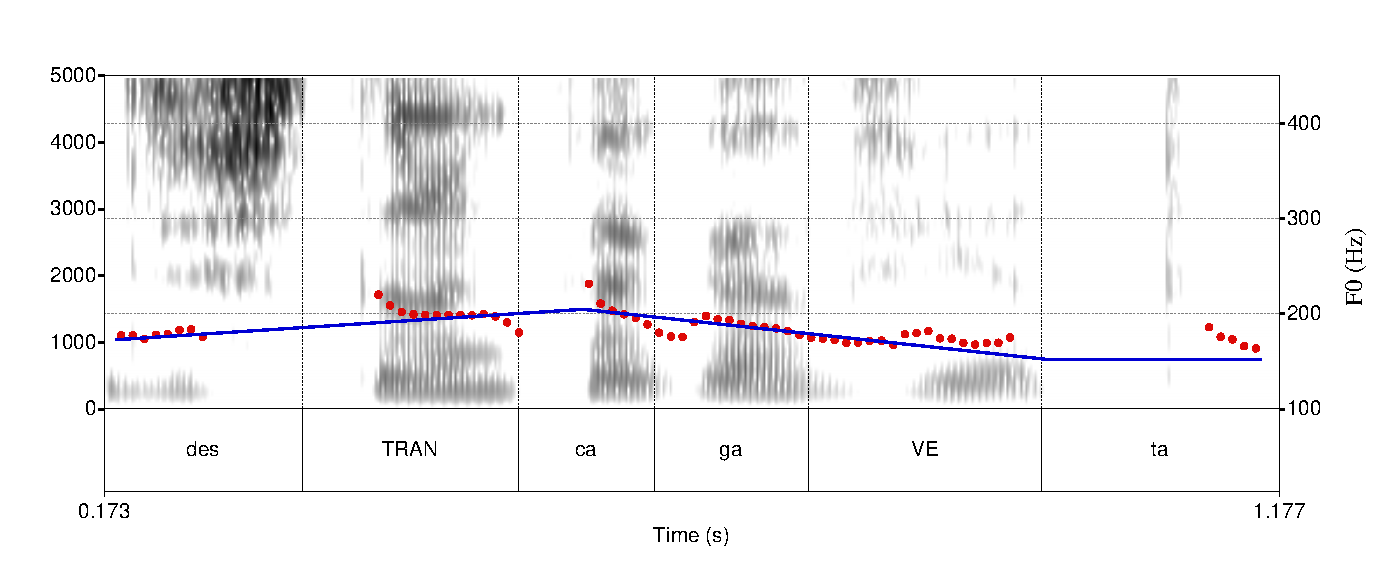
\includegraphics[width=0.99\textwidth]{figures/MOR3.eps}
\caption{Representation of the sentence \textit{Destranca a gaveta}, produced as a speech act of  the \textit{asserção} type -- as in an answer to \textit{O que ele faz quando chega em casa?} (`What does he do when he gets home?'): Spectrogram of the recorded sound (scale in Hertz on the left), measures of F0 estimated from the signal indicated by red dots and close-copy stylization by continuous straight blue lines (in Hz, right scale); the syllabic segmentation is indicated on the bottom tier.}
\label{figure:CC1}
\end{figure}

A sentence produced as a simple declarative \textit{asserção} (see Figure ~\ref{figure:CC1}), without any further expressive variation, shows a reduced F0 span (the middle 80\% range spans 3.6 semitones for the female and 5.4 for the male speaker on the complete corpus), rising up to the first stressed syllable and then falling to the end of the sentence. 
In this configuration, the final stressed syllable bears a low level of F0 with a falling configuration, while the pre-stressed syllable has a higher pitch level. 
Post-stressed syllables show the lowest pitch levels, with lowest intensity and possibly devoicing or creak.


\subsubsection{\textit{Interrogação} (`Yes/No question')}

\begin{figure}

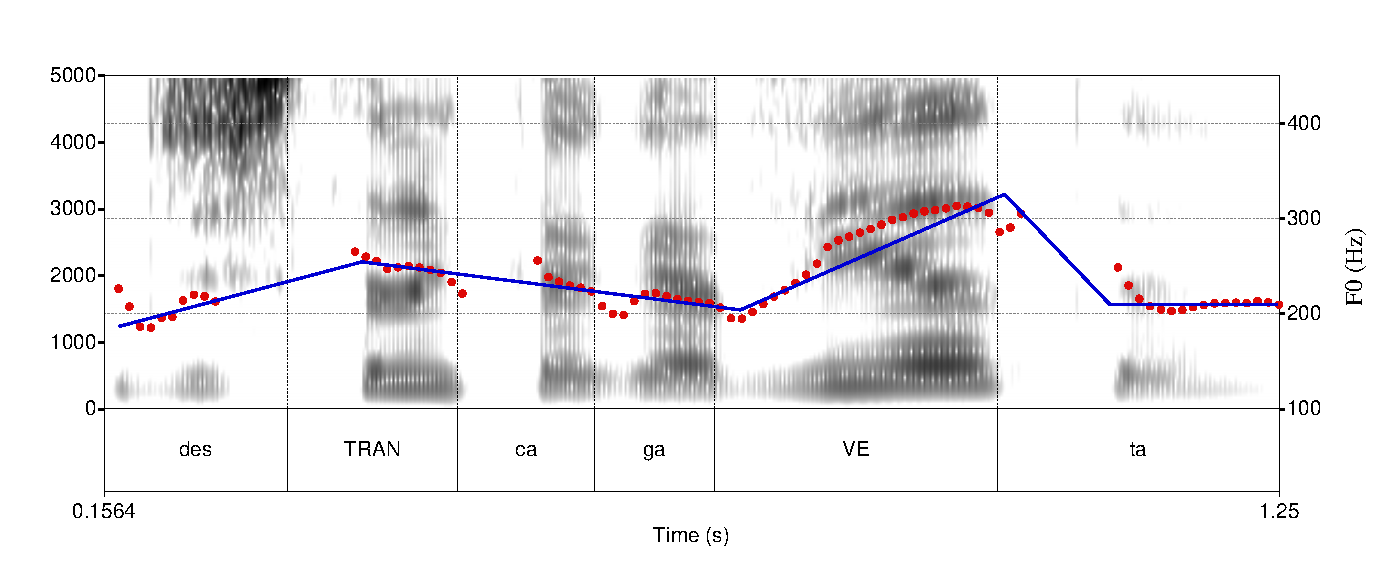
\includegraphics[width=0.99\textwidth]{figures/MOR4.eps}
\caption{Representation of the sentence \textit{Destranca a gaveta}, produced with a speech act of \textit{interrogação}: Spectrogram of the recorded sound (scale in Hertz on the left), measures of F0 estimated from the signal indicated by red dots and close-copy stylization by continuous straight blue lines (in Hz, right scale); the syllabic segmentation is indicated on the bottom tier.}
\label{figure:CC2}
\end{figure}

The sentence produced as an interrogative speech act (\textit{interrogação} -- see Figure~\ref{figure:CC2}) shows a wider F0 span (the middle 80\% range spans 8.2 semitones for the female and 11.4 for the male speaker on the complete corpus), presenting a double rising movement: The first (and the smallest) in the prenuclear position, and a second one in the nuclear position, reaching the highest level of the sentence in a rising movement along the final stressed syllable (not falling, like in \textit{asserção}) -- that is, the F0 peak has a late alignment. 
F0 then goes down on the potential post-stressed syllables. 
The valley between these two peaks is at its lowest at the end of the pre-stressed syllable.


\subsubsection{\textit{Ordem} (`order')}


\begin{figure}

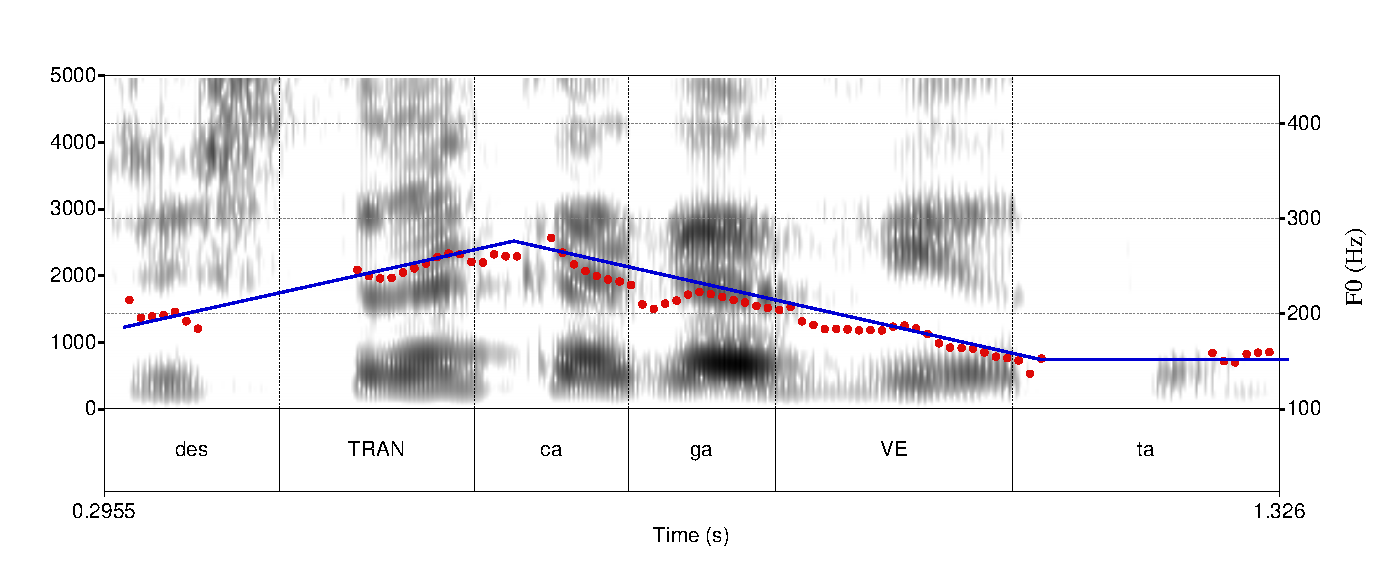
\includegraphics[width=0.99\textwidth]{figures/MOR5.eps}
\caption{Representation of the sentence \textit{Destranca a gaveta}, produced as a speech act of \textit{ordem}: spectrogram of the recorded sound (scale in Hertz on the left), measures of F0 estimated from the signal indicated by red dots and close-copy stylization by continuous straight blue lines (in Hz, right scale); the syllabic segmentation is indicated on the bottom tier.}
\label{figure:CC3}
\end{figure}

The expression of \textit{ordem} (Figure~\ref{figure:CC3}) shows a rising–falling movement: F0 rises along the prenuclear part, reaching the sentence's highest level on the first stressed syllable, and then falls until the nuclear position; the pitch span reaches medium levels (the middle 80\% range spans 7.7 semitones for the female and 14.0 for the male speaker on the complete corpus). 
The final stressed syllable is performed with a low pitch and a falling configuration, while the pre-stressed syllable has a higher pitch. 
Potential post-stressed syllables have the lowest F0 values.

\subsubsection{\textit{Desafio} (`threat, challenge')}

\begin{figure}

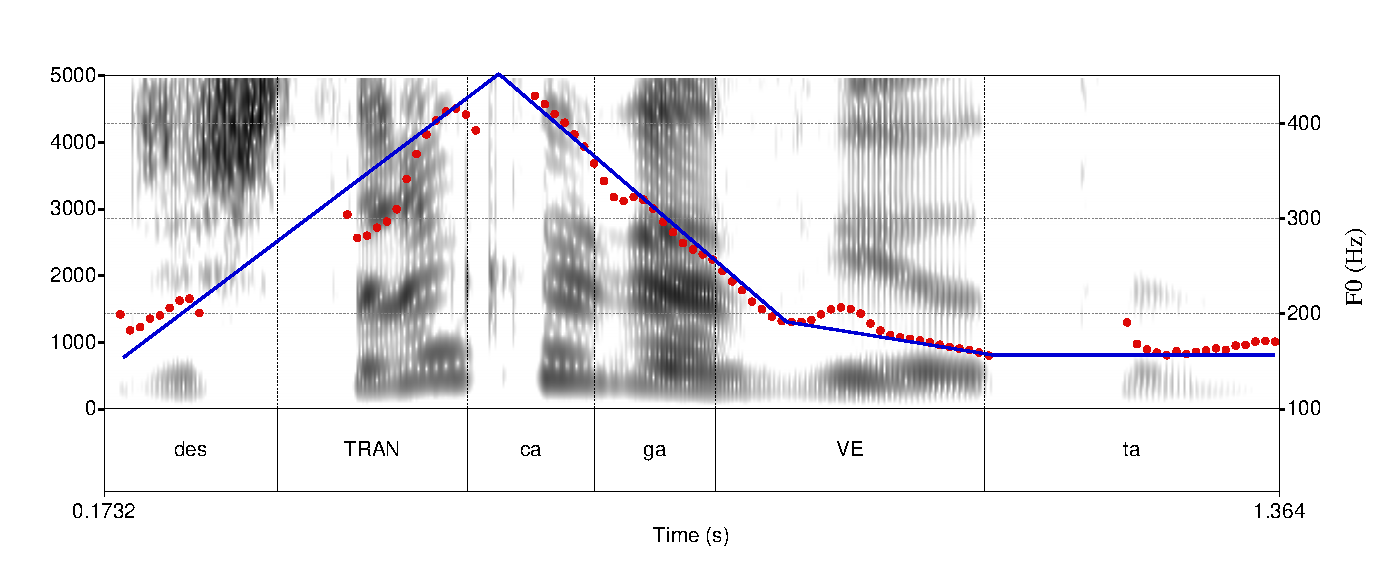
\includegraphics[width=0.99\textwidth]{figures/MOR6.eps}
\caption{Representation of the sentence \textit{Destranca a gaveta}, produced as a speech act of \textit{desafio}: Spectrogram of the recorded sound (scale in Hertz on the left), measures of F0 estimated from the signal indicated by red dots and close-copy stylization by continuous straight blue lines (in Hz, right scale); the syllabic segmentation is indicated on the bottom tier.}
\label{figure:CC4}
\end{figure}

\textit{Desafio}, as \textit{ordem} and \textit{asserção}, also shows a global rising–falling F0 contour (Figure~\ref{figure:CC4}): The movement rises during the prenuclear part, up to the end of the first stressed syllable, and goes down until the nuclear position. 
Differing from \textit{asserção} and \textit{ordem}, \textit{desafio} receives the largest pitch span (the middle 80\% range spans 17.1 semitones for the female and 23.2 for the male speaker on the complete corpus), with an especially high rise in the first stressed syllable. 
The final stressed syllable shows a falling configuration, at the end of the falling contour. 
The eventual post-stressed syllables receive the lowest F0 values. 
The change in the slopes of the falling contour on the pre-stressed syllables, compared to the stressed syllable, is not relevant as far as speech acts are concerned.


\subsubsection{\textit{Alerta} (`warning')}
\label{corpus:warning}

\begin{figure}

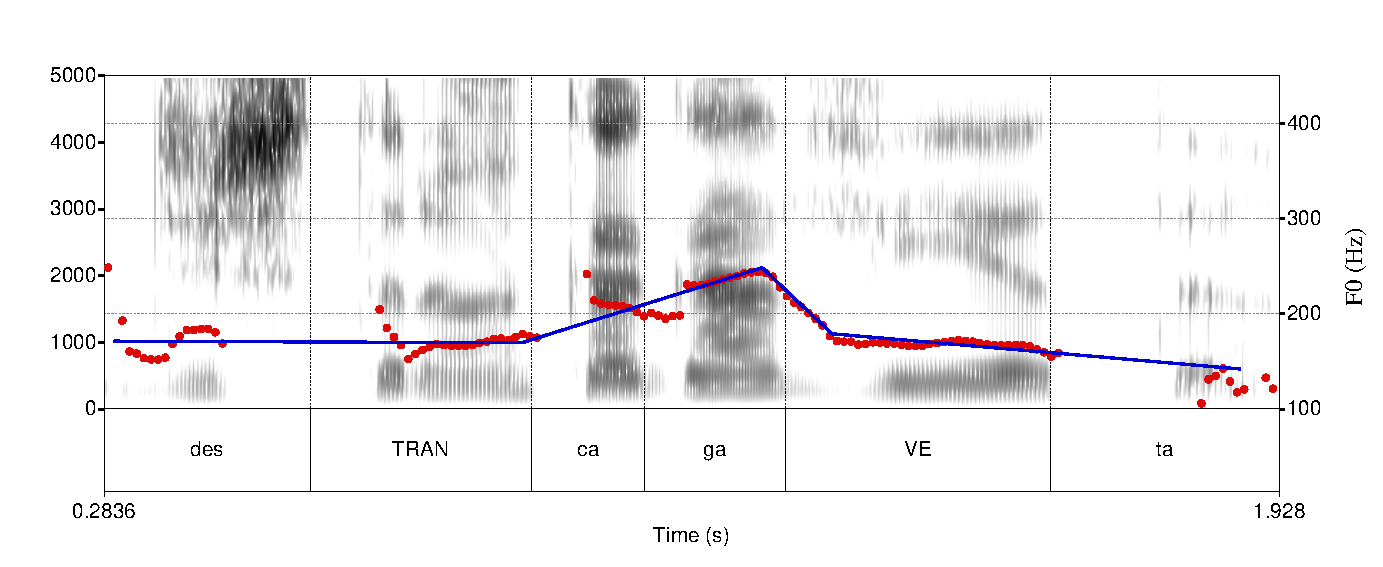
\includegraphics[width=0.99\textwidth]{figures/MOR7.eps}
\caption{Representation of the sentence \textit{Destranca a gaveta}, produced as an \textit{alerta} speech act: Spectrogram of the recorded sound (scale in Hertz on the left), measures of F0 estimated from the signal indicated by red dots and close-copy stylization by continuous straight blue lines (in Hz, right scale); the syllabic segmentation is indicated on the bottom tier.}
\label{figure:CC5}
\end{figure}

The intonation contour for the expression of \textit{alerta} (Figure~\ref{figure:CC5}) may also be summarized as a rising–falling one, but it does not follow the same timing as those observed for \textit{asserção}, \textit{ordem} and \textit{desafio}: Unlike those, the rise for \textit{alerta} starts later, after the first stressed syllable, and ends just before the final stressed syllable. 
The F0 movement spans a notable F0 range (the middle 80\% range spans 8.4 semitones for the female and 12.5 for the male speaker on the complete corpus). 
The pitch movement on the final stressed syllable is descending down to the post-stressed syllable, with a sharp fall at the beginning and an important lengthening of the stressed syllable (with a median duration in \textit{alerta} of 0.551 and 0.604 seconds for the female and male speakers respectively, vs. median durations in \textit{asserção} of 0.308 and 0.253 seconds for the female and male speakers). 
The potential post-stressed syllable continues this descending movement down to the lowest F0 in the sentence.


\subsubsection{\textit{Sugestão} (`suggestion')}

\begin{figure}

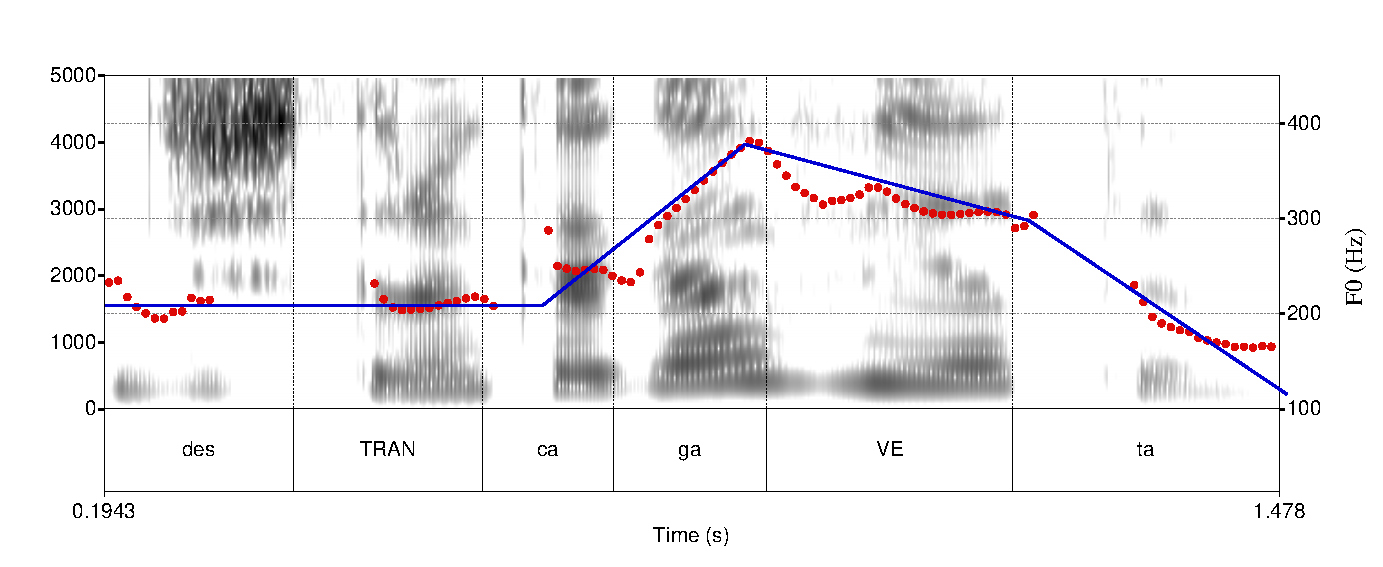
\includegraphics[width=0.99\textwidth]{figures/MOR8.eps}
\caption{Representation of the sentence \textit{Destranca a gaveta}, produced as a speech act of \textit{sugestão}: Spectrogram of the recorded sound (scale in Hertz on the left), measures of F0 estimated from the signal indicated by red dots and close-copy stylization by continuous straight blue lines (in Hz, right scale); the syllabic segmentation is indicated on the bottom tier.}
\label{figure:CC6}
\end{figure}

Expression of \textit{sugestão} (Figure~\ref{figure:CC6}), like that for \textit{alerta}, presents a rising–falling contour with a late rise, spanning the two unstressed syllables between the stress in prenuclear position, up to the final one. 
The melodic movement is wider than for \textit{alerta} (the middle 80\% range spans 10.8 semitones for the female, and 12.4 for the male speaker on the complete corpus). 
After the F0 peak, the melodic movement shows a light fall on the stressed syllable that stays at a high level, and a steep fall on the post-stressed syllable, departing from \textit{alerta}. 
\textit{Sugestão} also departs from \textit{alerta} in terms of lengthening -- lacking the typical lengthening  on the final stressed syllable observed in \textit{alerta}.


\subsubsection{\textit{Pedido} (`request')}

\begin{figure}

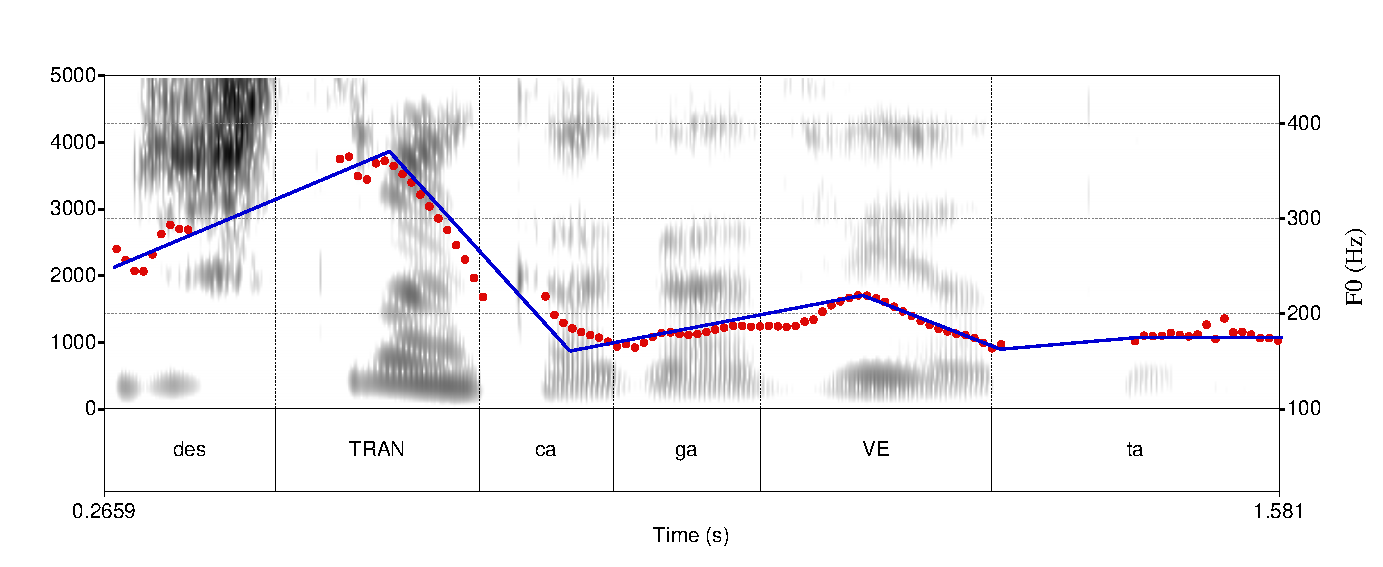
\includegraphics[width=0.99\textwidth]{figures/MOR9.eps}
\caption{Representation of the sentence \textit{Destranca a gaveta}, produced as a speech act of \textit{pedido}: Spectrogram of the recorded sound (scale in Hertz on the left), measures of F0 estimated from the signal indicated by red dots and close-copy stylization by continuous straight blue lines (in Hz, right scale); the syllabic segmentation is indicated on the bottom tier.}
\label{figure:CC7}
\end{figure}

Finally, the expression of \textit{pedido} depicts a double rise (one on each stressed syllable, see Figure~\ref{figure:CC7}), and is similar in that respect to the \textit{interrogação} expression. 
The first rise, on the stressed syllable at the prenuclear position, reaches the highest level -- contrary to the \textit{interrogação} contour. 
The second rise is located on the nuclear stressed vowel. 
Both peaks are located at the beginning of the vowels (early alignment), thus leading to a falling F0 contour during the stressed vowels. 
The valley between these two peaks is at its lowest at the end of the first post-stressed syllable; this also differs from the \textit{interrogação} contour, with a much steeper slope in \textit{pedido}, spanning the first stressed syllable and its post-stressed syllable, followed by a shallower rise up to the nuclear stress. 
The final post-stressed syllable bears a low tone. 
The F0 span is of 12.0 semitones for the female and 17.1 for the male speaker on the complete corpus (middle 80\% range).


\subsection{Close-copies of intonation contours}
\label{corpus:CC}

In order to explore similarities and differences between these contours, the notion of close-copy, developed by 't Hart and colleagues at IPO was used \citep{hart1991jasa}. 
It basically consists of a straight-line stylization of the raw F0 contour, using as few straight lines as needed so as to obtain a perceptually indistinguishable stimulus. 
Close-copies were obtained here using the stylization capabilities of Praat (its ``Stylize pitch'' function, used with a threshold of two semitones), and then reaching a minimal number of straight lines by hand, thanks to a careful process of listening. 
This concept of close-copy is the basis of other processes of intonation stylization, which reach perceptually identical stimuli by means of, for example, quadratic splines (for MOMEL, cf. \citealt{Hirst1993}) or straight-line stylization of vocalic nucleus (the model of tonal perception proposed by \citealt{dAlessandro1995tonal}, implemented into the \textit{Prosogram} by \citealt{mertens2004outil}). 
The lines that constitute the close-copies of each of these seven expressions are presented in Figures~\ref{figure:CC1} to~\ref{figure:CC7} (the straight lines that approximate the raw F0 estimation). 
The notion of equivalent-copy -- the intonation contour of a close-copy simplified even more so as to reach a stimulus that, if not perceptually identical to the original, does not lead to any difference in its interpretation -- is then used to simplify further the contours of these expressions.

The phonetic description of these seven speech acts (cf. the preceding part) leads to three types of contours: 
\begin{enumerate}
\item rising–falling contours with a peak near the end of the prenuclear stressed syllable (and thus a rise during the first stress and a slope on the second stress); 
\item rising–falling contours with a peak reached at the end of the pre-stressed syllable (nuclear stress) -- and thus a rise along the unstressed part of the sentences between the stressed syllables; and 
\item two-peak contours, observed on the two accented syllables (the details of these two-peak contours will be analyzed later).
\end{enumerate}

These three categories of contours present equivalent-copies that share striking similarities -- as well as some differences.


\begin{figure}[t]
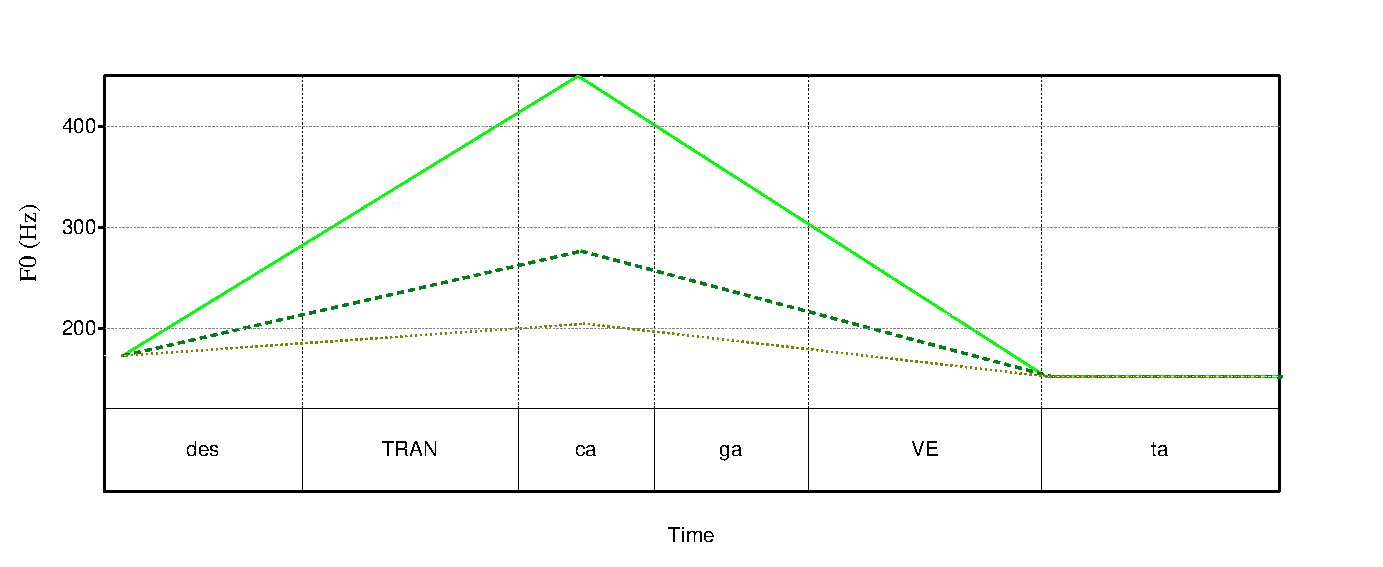
\includegraphics[width=0.99\textwidth]{figures/MOR10.eps}
\caption{Equivalent-copies of the speech acts of \textit{asserção} (dotted curve), \textit{ordem} (dashed curve), and \textit{desafio} (plain lines); the alignment of contours onto the phonetic segments is normalized to remove variation in timing between the expression and projected onto the segmentation of \textit{asserção} (time-normalization is done at the level of syllable).}
\label{figure:EC1}
\end{figure}

The first category regroups \textit{asserção}, \textit{ordem}, and \textit{desafio} (Figure~\ref{figure:EC1}). 
They are distinguished mostly by the span of the F0 peaks, as one can observe in Figure~\ref{figure:EC1}, representing the time-normalized equivalent-copies of these three speech acts. 
The similarities of the three contours are obvious, as are their clear differences in terms of F0 spans. 
The alignment of the contours on the segmental content is comparable, as are the initial and final F0 levels of each contour.

\begin{figure}[t]
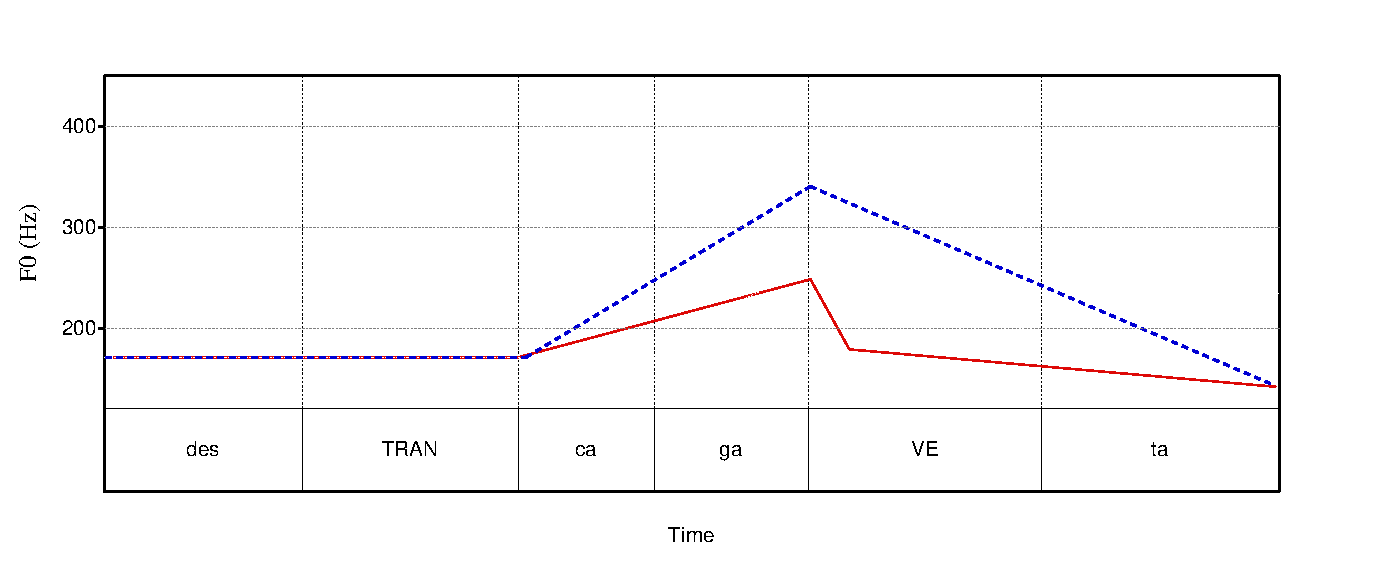
\includegraphics[width=0.99\textwidth]{figures/MOR11.eps}
\caption{Equivalent-copies of the speech acts of \textit{sugestão} (dashed curve) and \textit{alerta} (plain lines); the alignment of contours onto the phonetic segments is normalized to remove variation in timing between the expression and projected onto the segmentation of \textit{asserção} (time normalization is done at the level of syllable).}
\label{figure:EC2}
\end{figure}

The second category regroups the \textit{sugestão} and \textit{alerta} expressions, both of which have a rising–falling contour with a late rise, starting after the prenuclear stress, up to the nuclear stress. 
Figure~\ref{figure:EC2} shows their two equivalent-copies. 
One can observe that the two rises differ, as between the expressions in the first group, in terms of pitch span but not in their segmental anchoring. 
The main difference, though, is linked with the falling parts, which mostly span the nuclear stressed syllable. 
\textit{Sugestão} shows a continuous straight line from the beginning of the stressed syllable down to the end of the sentence, while \textit{alerta} has a typical sharp F0 fall at the beginning of the stressed syllable (mostly on the consonant part), followed by a shallow slope through the stressed vowel, down to the end of the sentence.


\begin{figure}

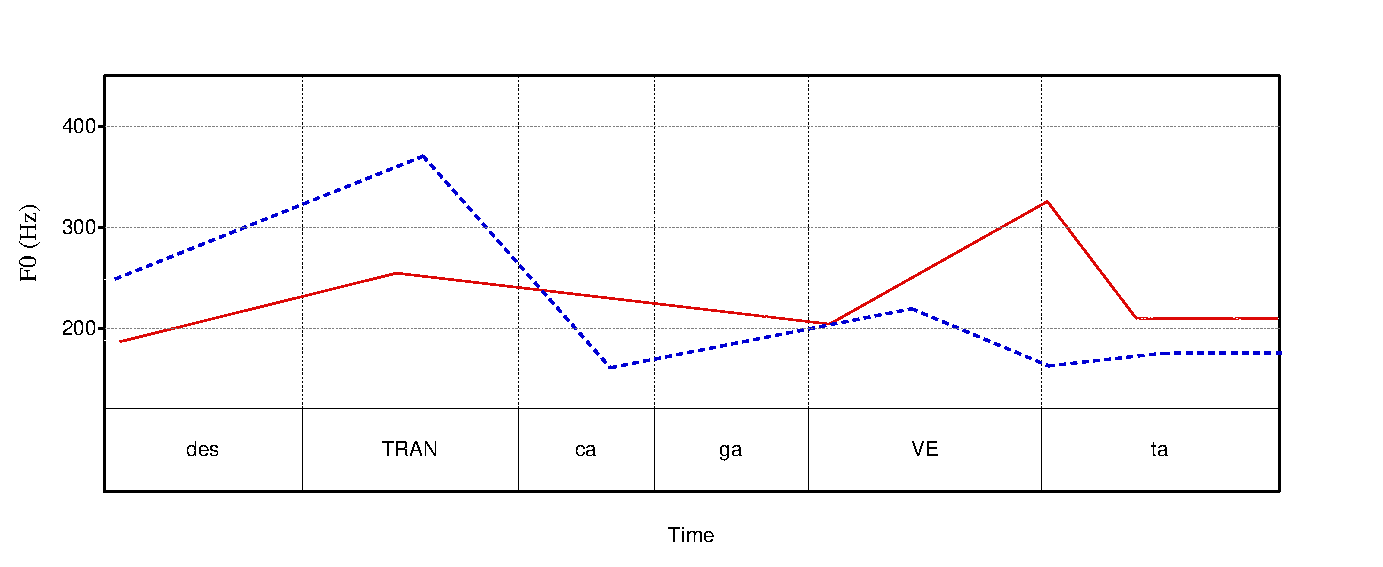
\includegraphics[width=0.99\textwidth]{figures/MOR12.eps}
\caption{Equivalent-copies of the speech acts of \textit{pedido} (dashed curve) and \textit{interrogação} (plain lines); the alignment of contours onto the phonetic segments is normalized to remove variation in timing between the expression and projected onto the segmentation of \textit{asserção} (time normalization is done at the level of syllable).}
\label{figure:EC3}
\end{figure}

The third category, with \textit{interrogação} and \textit{pedido}, regroups two-peak contours, one on each stressed syllable (see Figure~\ref{figure:EC3}). 
Apart from the presence of peaks on these two syllables, the contours have many differences, including differences in pitch span (first peak higher for \textit{pedido}, second for \textit{interrogação}) and differences in segmental anchoring (the second peak of \textit{interrogação} has a late alignment, while \textit{pedido} is aligned to the start of the stressed vowel; the valley between the two peaks reaches its minimum at the start of the nuclear stressed syllable for \textit{interrogação} but during the first prenuclear post-stressed syllable for \textit{pedido}).

The determination of the equivalent-copies underlines the potential interest of two types of parameters in these performances: 
(1) the number of pitch levels; 
and (2) the segmental anchoring of peaks and valleys.
These two parameters notably change the slopes, direction, and steepness on the stressed vowels.

\subsection{Importance of other acoustic parameters of prosody}
\label{corpus:importance}

Equivalent-copies focus on the melodic contour as the main dimension to express such speech acts. 
If fundamental frequency is certainly a major parameter for prosodic expression, intensity and duration also play a role (see \citealt{kochanski2005loudness}, for example). 
To that end, the use of stylization is interesting, as the stylized melodic contours can be transferred onto another sentence, with a similar segmental content but different duration, intensity, and voice quality. 
This is achieved by mixing, for example, a sentence's melody -- let's say with a \textit{pedido} pitch contour -- with the \textit{asserção} sentence's segments, following the process schematized in Figure~\ref{figure:Transplantation}; the equivalent copy (thus the melodic contour) of \textit{pedido} (lower left graph) is transferred onto the \textit{asserção} (upper left graph), keeping a proportional segmental anchoring of straight lines' beginning and end at the syllable level. 
This is achieved thanks to Praat's ``Manipulation'' object, and the result is presented in the right graph. 
The resulting sound has the temporal, intensity, and articulation patterns of \textit{asserção}, but the melodic contour of \textit{pedido} (note that one may also have mixed the duration and intensity parameters using a similar procedure).


\begin{figure}

\includegraphics[width=0.99\textwidth]{figures/MOR13.eps}
\caption{Schematic representation of transplanting the melodic contour of one sentence onto another: On the left, the two original sentences (top: \textit{asserção}, bottom: \textit{pedido}) showing the same segments but different prosodic parameters (each graph presents, over the spectrogram, the raw pitch in speckles, the intensity in curved lines, and the close-copy stylization of intonation in straight lines); on the right, the result of transplanting the melodic curve of \textit{pedido} onto the segmental content of \textit{asserção}.}
\label{figure:Transplantation}
\end{figure}


\section{Perception tests}
\label{perception}

To validate the importance of various aspects of the melodic contours described above, perception tests were carried out. 
The first test aimed to validate that each original performance expresses a speech act that is distinguishable from the others and recognized for what it was intended to express; a categorical perception test was thus run on the natural stimuli, the subjects having to judge the intended speech act among the five categories (\textit{ordem}, \textit{pedido}, \textit{alerta}, \textit{sugestão}, and \textit{desafio} -- the neutral \textit{asserção} and \textit{interrogação} were not part of the test).


\subsection{Categorical recognition}
\label{perception:categorical}

The categorical recognition test was taken by 34 subjects, native speakers of BP, who had to identify the intended speech act among the five possible acts. 
The stimuli were based on five sentences with varying length (one, three, six, nine and 12 syllables), each sentence produced by one female speaker with the five speech acts (thus resulting in 25 stimuli). 
All sentences but the one with a single syllable were based on a final word bearing a paroxytonic stress. 
The percentages of correct recognition (presented in Figure~\ref{figure:reco}) were then analyzed (complete results, based on more speakers and expressions, are presented in \citealt{moraes2014}). 
As recognition scores are binary data, a logistic regression was applied (following \citealt[][196]{baayen2008analyzing}, and using R's glm() procedure; \citealt{Rtool}). 
The predictors used to fit the results were the presented speech act (five levels) and the support sentence (five levels), plus the interaction between both factors.


\begin{figure}

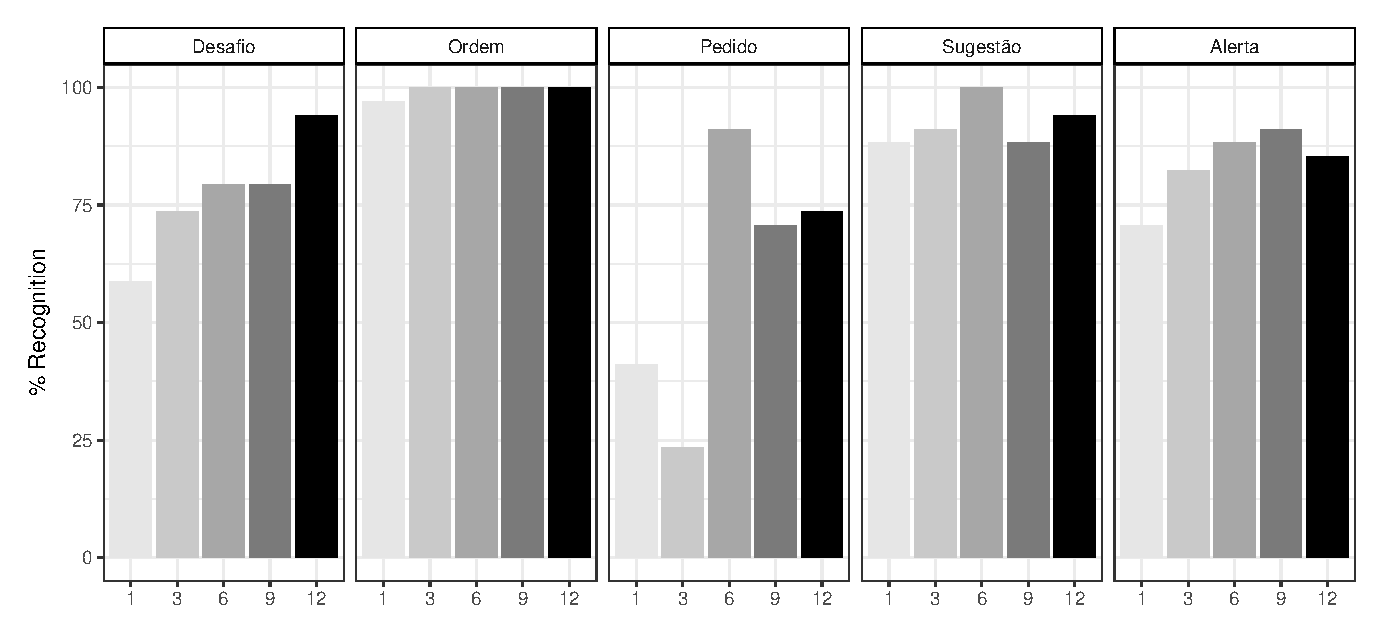
\includegraphics[width=0.99\textwidth]{figures/MOR14.eps}
\caption{Bar graph representing the recognition percentages obtained by each of the 25 stimuli (five sentences performed with five speech acts); each box presents the results for one speech act, with the five sentences ranked by length.}
\label{figure:reco}
\end{figure}

\begin{table}
\caption{Output of the logistic regression on the categorical perception results: Likelihood ratio test against the chi square distribution ($LR \chi^2$), degrees of freedom (\textit{df}) and observed probability ($p$).}
\label{tab:binom}
 \begin{tabular}{lSSS} % add l for every additional column or remove as necessary
  \lsptoprule
            & \multicolumn{1}{c}{$LR \chi^2$}  &  \multicolumn{1}{c}{\textit{df}}  &  \multicolumn{1}{c}{$p$} \\
  \midrule
Speech act  &  127.2  &  4  &  < 0.0001 \\
Sentence  &  46.8  &  4  &  < 0.0001 \\
Speech act * Sentence  &  27.7  &  16  &  < 0.05 \\
  \lspbottomrule
 \end{tabular}
\end{table}

Results of the logistic regression (see Table~\ref{tab:binom}) show that all factors have a significant effect on the recognition of speech acts. 
The factor speech act has the largest effect, with \textit{pedido} and \textit{desafio} receiving the lowest recognition scores. 
As one can observe in Figure~\ref{figure:reco}, this is mainly due to the short sentences (one and three syllables long), and similarly, the effect of sentence length is mostly due to poor recognition scores in short sentences, mainly observed in the expressions of \textit{pedido} and \textit{desafio} (thus the significant interaction). 
From this set of sentences, the one that is analyzed in the preceding section is the six-syllable sentence, which receives high recognition scores for all speech acts.

\subsection{Quality of the performance}
\label{perception:performance}

The close-copy stylizations of the intonation pattern typical of each expression were produced from the six-syllable sentences (see Section~\ref{corpus}). 
From such stylization, one may test two aspects of prosody: The perceptual importance of a given stylization parameter (in terms of melodic level or segmental anchoring) for the understanding of a given speech act, and the relative role of pitch versus intensity and duration in conveying a given expression. 
To test these two aspects, we will describe here a perception test that focuses on the third group of intonation contours described in Section~\ref{corpus:CC}: The two-peak contours observed for the expressions of \textit{interrogação} and \textit{pedido}. 
Several questions may be raised about these contours to have a better understanding of the parameters important for their expression:
\begin{itemize}
\item Minimum number of pitch levels useful for reproducing these expressions;
\item Temporal anchoring of intonation contours regarding the segmental structure of the sentence;
\item Importance of pitch versus the other prosodic dimensions (loudness, duration).
\end{itemize}

To test these three points, several resyntheses of the two close-copies were produced by altering various components of their structure:
\begin{itemize}
\item Transplanting the stylized intonation contour onto the neutral \textit{asserção} sentence to remove any intensity and duration changes that could help in characterizing these two expressions.
\item Averaging the pitch levels of the two expressions, for various parts of the contours, to test the extent to which the pitch level plays a role at a given position in the sentence.
\item Changing the segmental anchoring of the pitch contours to observe whether the pitch alignment changes the understanding of expressions.
\end{itemize}

With such aims and modifications, 48 stimuli were produced (24 for each of the two speech acts), on the basis of the 12 modifications described hereafter, and resynthesized using either the original segmental information (from \textit{pedido} or from \textit{interrogação}), or the segmental information of \textit{asserção}. 
The close-copy stylizations of \textit{interrogação} (`yes/no question') and \textit{pedido} (`request') are reproduced in Figure~\ref{figure:TP}, with labels associated with each end of the stylized pitch segments; these points are modified in the following way:
\begin{description}
\item [M1:] The original close-copy reproduction of both expressions.
\item [M2:] P1 averaged for frequency in both contours.
\item [M3:] P2 (initial peaks) averaged for frequency in both contours.
\item [M4:] P3 averaged for frequency in both contours.
\item [M5:] P4 (final peaks) averaged for frequency in both contours.
\item [M6:] P5 and P6 averaged for frequency in both contours.
\item [M7:] P3's segmental anchoring temporally averaged in both contours.
\item [M8:] P3's segmental anchoring inverted between the two contours (i.e., segmental anchoring of the \textit{interrogação} sentence P3 replaced by that of \textit{pedido}, and vice versa).
\item [M9:] P4's segmental anchoring inverted between the two contours (i.e., segmental anchoring of the \textit{interrogação} sentence's final peak replaced by that of \textit{pedido}, and vice versa).
\item [M10:] Averaging of frequency between both contours for each point in unaccented syllables (P1, P3, P5, P6).
\item [M11:] Averaging of frequency between both contours for each point (P1 to P6). Point P4b in the contour of \textit{pedido} is given P5's averaged frequency.
\item [M12:] The same averaging process for frequencies as in the preceding modification, plus averaging of the segmental anchoring of unaccented syllables (P1, P3, P5, P6). The point P4b of \textit{pedido} is removed. The two contours are similar for all their characteristics except for the segmental anchoring of peaks (P2, P4).
\end{description}

\begin{figure}

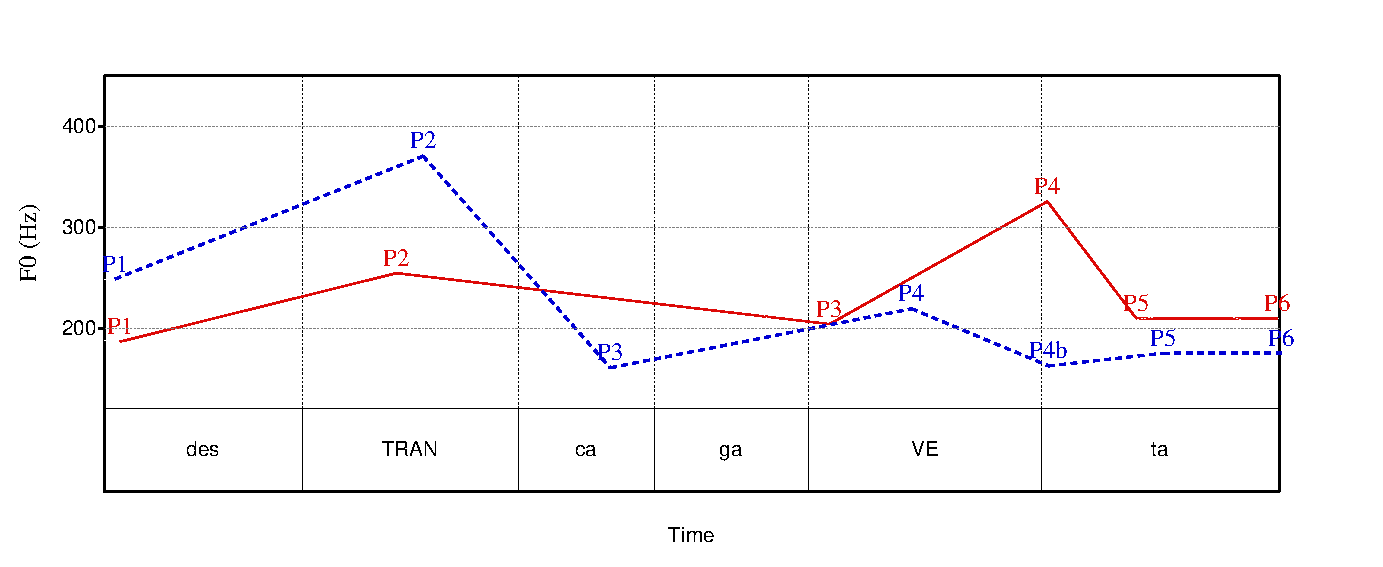
\includegraphics[width=0.99\textwidth]{figures/MOR15.eps}
\caption{Target points of the close-copy stylization of \textit{interrogação} (continuous line) and \textit{pedido} (dashed line).}
\label{figure:TP}
\end{figure}

\begin{table}
\caption{Results of the analysis of variance run on the quality measure: Effect of each factor and interactions among factors. Columns present the degrees of freedom (\textit{df}) of factors, the associated $F$ value, the $p$-value, and effect size ($\eta^2$).}
\label{tab:anova}
 \begin{tabular}{l *{4}{S}} % add l for every additional column or remove as necessary
  \lsptoprule
            & \multicolumn{1}{c}{\textit{df}}  & \multicolumn{1}{c}{$F$ value}  &  \multicolumn{1}{c}{$p$}  &  \multicolumn{1}{c}{$\eta^2$} \\
  \midrule
Modif                             &  11  &  15.95  &  <0.0001  &  0.142  \\
Speech act                                 &  1  &  17.95  &  <0.0001  &  0.017  \\
Segment                        &  1  &  192.22  &  <0.0001  &  0.154  \\
Modif * Speech act                     &  11  &  3.82  &  <0.0001  &  0.038  \\
Modif * Segment            &  11  &  0.76  &  0.680  &  0.008  \\
Speech act * Segment                &  1  &  2.16  &  0.142  &  0.002  \\
Modif * Speech act * Segment    &  11  &  2.83  &  <0.01  &  0.029  \\
Residuals                       &  1056  &    &    &  \\
  \lspbottomrule
 \end{tabular}
\end{table}

The 12 modifications (on two segmental substrates) obtained for \textit{interrogação} (and \textit{pedido}) were then presented to 23 subjects -- speakers of Rio de Janeiro BP--who had to judge if each stimulus was a good performance for \textit{interrogação} (and \textit{pedido}), on a scale of 1 to 5. 
An analysis of variance was then run on these scores, with three factors: The type of modification imposed on the stimulus (12 levels), the segmental substrate used to synthesize the stimulus (two levels) and the original speech act (two levels). 
Interactions (double and triple) between these factors were also tested. 
The results are presented in Table~\ref{tab:anova}.



The mean values of the quality judgments given to each stimulus are depicted in Figure~\ref{figure:Quality}. 
The reference level of a good quality for each expression is given by the two close-copies (M1) on the original segmental substrate. 
Post-hoc Tukey tests allowed for testing the significance of differences in quality perceived between pairs of modifications; they show the following significant differences:
\begin{itemize}
\item Among stimuli based on the original segmental substrate:
\begin{itemize}
\item For \textit{interrogação}: M8, M11, and M12 modifications received significantly lower scores than M1.
\item For \textit{pedido}: M8, M9, M11, and M12 modifications received significantly lower scores than M1.
\end{itemize}
\item Among stimuli based on the neutral substrate:
\begin{itemize}
\item For \textit{interrogação}: M5, M8, M11, and M12 modifications received significantly lower scores than M1 neutral.
\item For \textit{pedido}: No modification received a significantly different score compared to M1 neutral.
\end{itemize}
\item Between original and neutral-based M1 stimuli:
\begin{itemize}
\item The difference between the two \textit{interrogação} M1 modifications is not significant.
\item The difference between the two \textit{pedido} M1 modifications is significant.
\end{itemize}
\end{itemize}

\begin{figure}

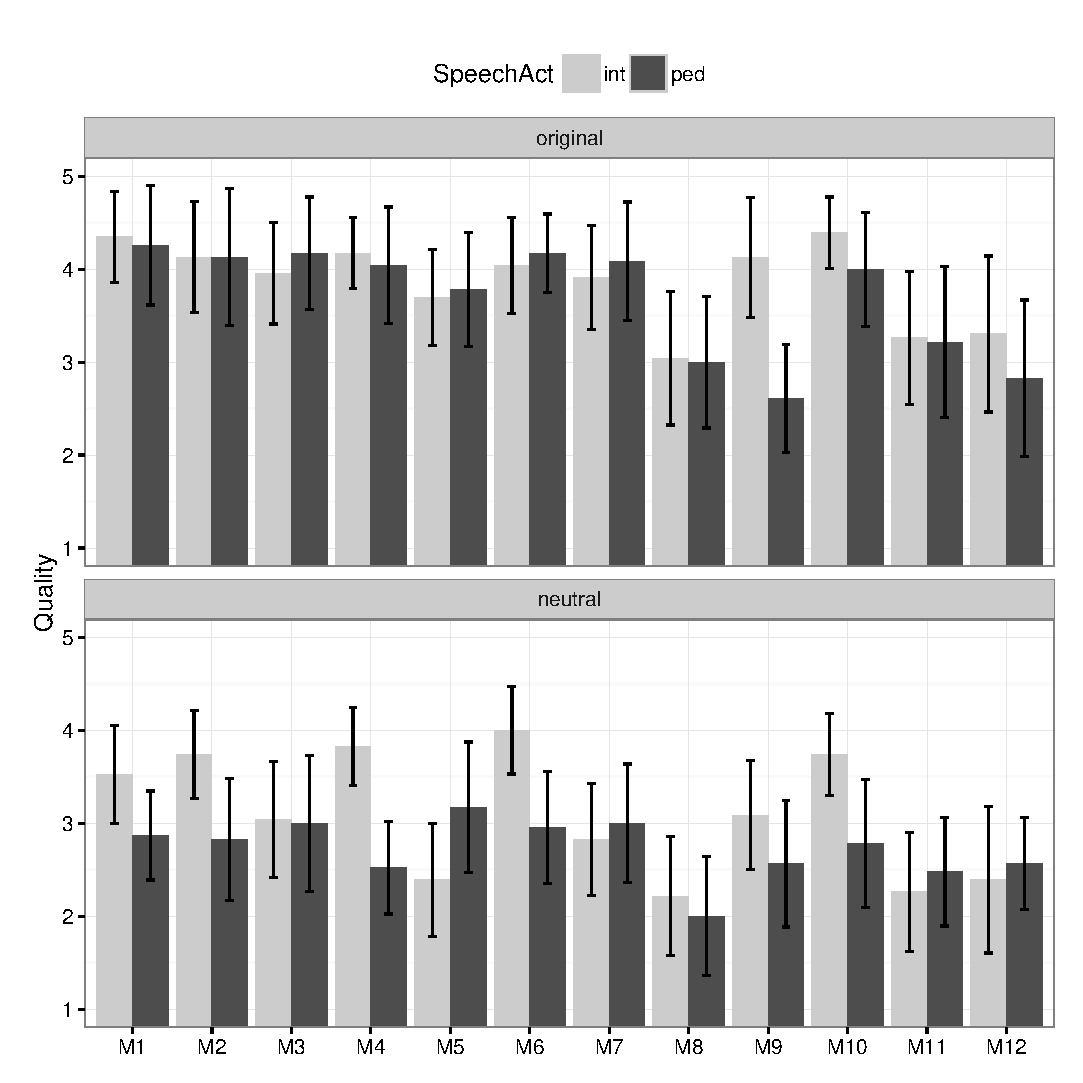
\includegraphics[width=0.99\textwidth]{figures/MOR16.eps}
\caption{Bar graphs representing the mean quality given to each of the 48 stimuli (two speech acts with 12 modifications, resynthesized on twop segmental bases).}
\label{figure:Quality}
\end{figure}


\section{Discussion}\label{discussion}\largerpage

Section~\ref{corpus} describes three categories of pitch contours, for speech acts in the Rio de Janeiro variety of Brazilian Portuguese.  
The first category bears a peak at the end of the prenuclear stress. 
Among the three performances of this category, \textit{asserção} conveys a simple statement without imposition of the speaker onto the hearer. 
By expressing \textit{ordem}, the speaker imposes on the listener her/his will. 
In \textit{desafio}, the speaker dares the listener to perform something; the speaker does not want the hearer to perform this act. 
This could be interpreted under the terms of \citet{Brown1987} as three speech acts with varying threats to each interlocutor's face: No threat for \textit{asserção}; a threat to the negative face of the hearer with \textit{ordem}; and, with \textit{desafio}, a threat by the speaker to the negative face of the hearer to dare, challenging the positive face of the speaker. 
For the speech acts of \textit{ordem} and \textit{desafio}, the speaker and the hearer are in a relation of dominance, with the speaker having power over the hearer \citep{spenceroatey1996power}. 
The second category regroups two contours with a peak observed later in the sentence (reaching its maximum at the beginning of the nuclear stress). 
These contours express directive speech acts (\textit{sugestão} and \textit{alerta}) with a speaker in a retracted position, showing less personal implication in the outcome compared to the preceding speech acts (there is no threat on the speaker’s face in these cases). 
The third category regroups contours performed with two peaks, one at the prenuclear and one at the nuclear position. 
These contours express two speech acts (\textit{interrogação} and \textit{pedido}) in which the speaker is somehow dependent on the listener. 
This could be interpreted as the speaker being in a lower position or having less power than the hearer \citep{spenceroatey1996power}. 
For \textit{interrogação}, the speaker is at least dependent on the hearer for having information \citep[see the interpretation of a ``desire for the goodwill of the receiver'' given in ][343]{ohala1994symbolism}.\largerpage

Speech acts inside each of these three groups thus share similarities in shape and in meaning. 
In the first group of speech acts, there is an increased imposition of the speaker onto the hearer, linked to a more dominant behavior or position. 
This seems to be reflected in the pitch span -- the wider the span, the stronger the imposition, following the mechanism of sound symbolism described by the \textit{Effort Code} for authority \citep{Gussenhoven2004}. 
The two speech acts of \textit{ordem} and \textit{desafio} are also performed with a relatively low base pitch (as compared to other speech acts; see Figure~\ref{figure:f0intbase}), in accordance with the \textit{Frequency Code}'s predictions for dominant expressions \citep{ohala1994symbolism}. 
Such a need to keep the pitch low (in comparison with ``neutral'' pitch) may explain the difference between the strategies of the female and the male speakers regarding \textit{ordem}. 
The female speaker has a base pitch for \textit{asserção} (i.e., the more neutral speech act) close to the mean of her base pitches, while the male speaker's base pitch for \textit{asserção} is low among his base pitches (see Figure~\ref{figure:f0intbase}). 
The female can lower her pitch while producing loud \textit{ordem}; the male speaker has to refrain from getting very loud in performing \textit{ordem} if he wants to keep the base pitch relatively low -- thus, the difference in median intensity and intensity span observed for \textit{ordem} between these two speakers.

The importance of the localization of the maximum pitch along the sentence (early, during the prenuclear part, or late, during the nuclear part) opposes speech acts that impose more (for early peaks) or less (for late maximum peaks) on the hearer. 
Early peaks are typical of the involved directives of the first group and of \textit{pedido} (the first peak of \textit{pedido} is higher than the second, contrary to \textit{interrogação}). 
Late peaks are typical of the second group (distanced directives) and of \textit{interrogação}. 
Such an analysis is in conformity with the \textit{Frequency Code}, which predicts that raised or rising pitch on an utterance would tend to carry a more submissive meaning \citep{ohala1994symbolism}. 
Distinctions inside these groups are made either in terms of power, imposition, or dominance (with the gradation of imposition levels presented in the first group) or in terms of shape for the second group (a sharp pitch fall after the peak vs. a plateau).

Then the importance of pitch alignment with the segmental substrate, the number of distinctive pitch levels, and the relative importance of other prosodic parameters (duration, intensity) required to adequately perform a given speech act have been investigated.

The relative importance of prosodic parameters in conveying such speech acts in Rio de Janeiro’s variety of BP is tested in transferring the melodic contours onto the neutral segmental substrate. 
The scores given by listeners to the resulting stimuli show that pitch alone is sufficient to express the speech act of \textit{interrogação} -- while the duration and intensity play a significant role for \textit{pedido}, in combination with F0. 
Duration is also mandatory in the expression of \textit{alerta} (see Section~\ref{corpus:warning}), in which the important lengthening of the final stressed syllable goes along with the melodic contour (note that the importance of duration in this case is not formally tested in this paper). 
The use of other parameters for expressive speech acts, and typically intensity, is linked to the notion of \textit{involvement} in speech described by \citet{danes1994involvement}, which refers to the illocutionary strength of the associated speech acts and thus to vocal effort \citep{Gussenhoven2004}. 
Intensity is known to be a primary correlate of increased vocal effort during speech production \citep{Lienard1999,Traunmuller2000}. 
But such changes are mostly linked to changes in the speaker's affective arousal \citep{Goudbeek2010} and induce changes in the mean levels of parameters -- that is, gradient differences -- derived from symbolic melodic gestures rather than conventional, arbitrary (hence phonological) signs \citep[cf.][]{bolinger1986intonation}.

If not the only expressive mean of prosody, melodic contours certainly bear a great deal of the prosodic speech acts' semantics in BP \citep{moraes2014}. 
In doing so, F0 variation expresses an additional meaning (a prosodic meaning because it is not necessarily expressed by morphosyntactic means) that changes the original utterance's literal meaning. 
This allows the speaker to address a question, a statement, an order, and so on, without resorting to lexicon. 
The codification of these prosodic speech acts obeys phonological rules depending on languages -- if possibly derived from symbolic codes \citep{ohala1983,bolinger1986intonation}.
The validity of the results presented here is, of course, limited to the Rio de Janeiro variety (one may even call into question possible sociocultural variation).
Meanwhile, this paper focuses on the methodological aspect, which may be used in further experiments to test the perception of these speech acts across dialectal varieties of BP -- or EP. 
We may speculate, given existing descriptions (cf. the introduction) and the level of diffusion through media of Rio de Janeiro’s variety of BP, that such speech acts will be recognized adequately within Brazil, showing variation comparable to the one observed within the two speakers described here (cross-gender variation, or for example variation due to personality; see \citealt{rilliard2016}).
Conversely, the EP varieties may show much different strategies, and possibly cross-cultural differences, in such performances -- but this has to be tested.


The two speech acts analyzed in detail in Section~\ref{perception:performance} share a global similarity, each presenting two peaks, one on each stressed syllable. 
But these peaks have distinct features in terms of pitch height and segmental anchoring that allow listeners to recognize each speech act. 
The modifications of these characteristics introduced via a resynthesis technique allowed us to test the perceptual relevance of these features for the expression of the two speech acts (hence for this speaker).

For the speech act of \textit{interrogação}, only modifications M8, M11, and M12 significantly lowered the perception score. 
For \textit{pedido}, modification M9 also received low scores. 
Modification M8, by changing the segmental anchoring of the valley between the two peaks, basically smoothed the final rise of the \textit{interrogação}'s melodic contour, and the slope of the first peak for the \textit{pedido} contour. 
This shows that the F0 slope, and not only the peak anchoring, has a pertinent effect on perception.
M11, averaging the pitch height of each point, removed the relative difference in height between the first and second peak. 
M12 removed even further information from M11, causing the two contours to be almost comparable except for the peaks' segmental anchoring. 
M9 inverted the segmental anchoring of the second peak; thus, the peak of \textit{pedido} arose at the end of the stressed vowel while the peak of \textit{interrogação} arose at the beginning of the stressed vowel. 
The M9 modification inverted the slope of the pitch contours on the last stressed vowel: It rose for \textit{pedido}, and went down for \textit{interrogação}. 
For the speech act of \textit{interrogação}, the height of the final peak (compared to the first peak, the second being higher) and the steepness of this final peak's rise appear to be critical. 
For \textit{pedido}, the critical characteristics are the relative height of the first peak (compared to the final peak, the second being lower), the steepness of the first peak's slope down the initial stress's vowel, and the direction of the slope on the final stress's vowel. 

These results confirm the distinctive nature of the two contours beyond their two-peak categorization. 
Speech acts of \textit{interrogação} in BP are characteristically recognized by their steep rise on the final stress syllable -- at least in the Rio de Janeiro variety. 
Expressions of \textit{pedido}, on the other hand, are characterized by two peaks on stressed syllables (the first higher than the second), with these vowels bearing falling melodic contours. 
This descending slope is typical of \textit{asserção} and strong directive speech acts, while the two-peak configuration refers to \textit{interrogação}.
This mixture of characteristics may lead to the interpretation of \textit{pedido}.
The results of the experiment also shed light on the importance of the F0 slope's steepness, a factor that is linked to the anchoring of \textit{both} peaks and valleys.
The M11 modification having a perceptual effect (linked to the relevance of pitch differences between the two peaks' height), this result supports the need for at least three tonal levels in describing such melodic contour (one for valley, and two for peaks).
Before concluding on the phonological differences existing between these potential three levels, more studies must be pursued, but the presented methodology allows for such strictly controlled perception tests.


\section{Conclusions}
\label{conclusions}
The presented methodology allows one to investigate phonological differences conveyed by prosody at the speech act level. 
An application of this methodology was made on a corpus of seven prosodic speech acts in the Rio de Janeiro BP variety and shows that they can be perceptually distinguished. 
These seven speech acts are performed with three types of melodic contours: With a peak on the first stress, with a peak before the final stress, or with two peaks. 
The detailed characteristics of the contours in each group (their pitch span and height, their segmental anchoring, or the shape of their melodic contours) allowed listeners to distinguish each speech act. 
On the basis of a methodology using close-copy stylization and systematic changes in the constituents of these stylized contours, it has then been shown that the segmental anchoring of peaks and valleys, as well as the relative levels of peaks, has critical importance for the intonation of speech acts.
\largerpage[-1]

Typically, it is mandatory to have three levels of pitch register to describe the melodic contours conveying varying directive speech acts. 
Segmental anchoring of the stylized contours' valleys, on the inter-stress syllables, has an influence on the pitch slope and is thus important for the quality of the output. 
The melodic contour along the stressed syllables must be falling for \textit{pedido}, while its direction is not mandatorily rising for BP interrogations; one may find falling contours on final stress for BP questions, as in confirmative yes-no questions or wh-questions \citep{moraes2008pitch}.
Such results may have implications (outside the focus of this paper) for phonological models of prosody, and typically within an autosegmental-metric approach \citep{Ladd2008}, where it is customary to stick with two tone levels (see \citealt{FacePrieto.2007,dimperio2010alignment}). 

{\sloppy
\printbibliography[heading=subbibliography,notkeyword=this]}
\end{document}
